\part{\gls{ohdmconverter} als PostgreSQL Projekt}
\chapter{Projektidee}
Die Grundidee von \gls{ohdm} ist immer noch die selbe, kurz es sollen \gls{osm} Daten um die Dimension Zeit erweitert werden. Auch bleiben die bestehenden Datenbankschemata gleich. Die größte Änderung ist die Implementierung.

\section{osm2inter}
Für den Import von \gls{osm} Dateien soll ein bestehendes Tool \gequote{\gls{osm2pgsql}}\cite{osm2pgsql} verwendet werden. \gls{osm2pgsql}\cite{osm2pgsql} ist dafür ausgelegt \gls{osm} Daten in eine PostGIS Datenbank zu importieren.

\begin{figure}[h]
	\caption{Entity Relationship Diagramm der \gls{inter} Datenbank}
	\label{fig:erd-inter}
	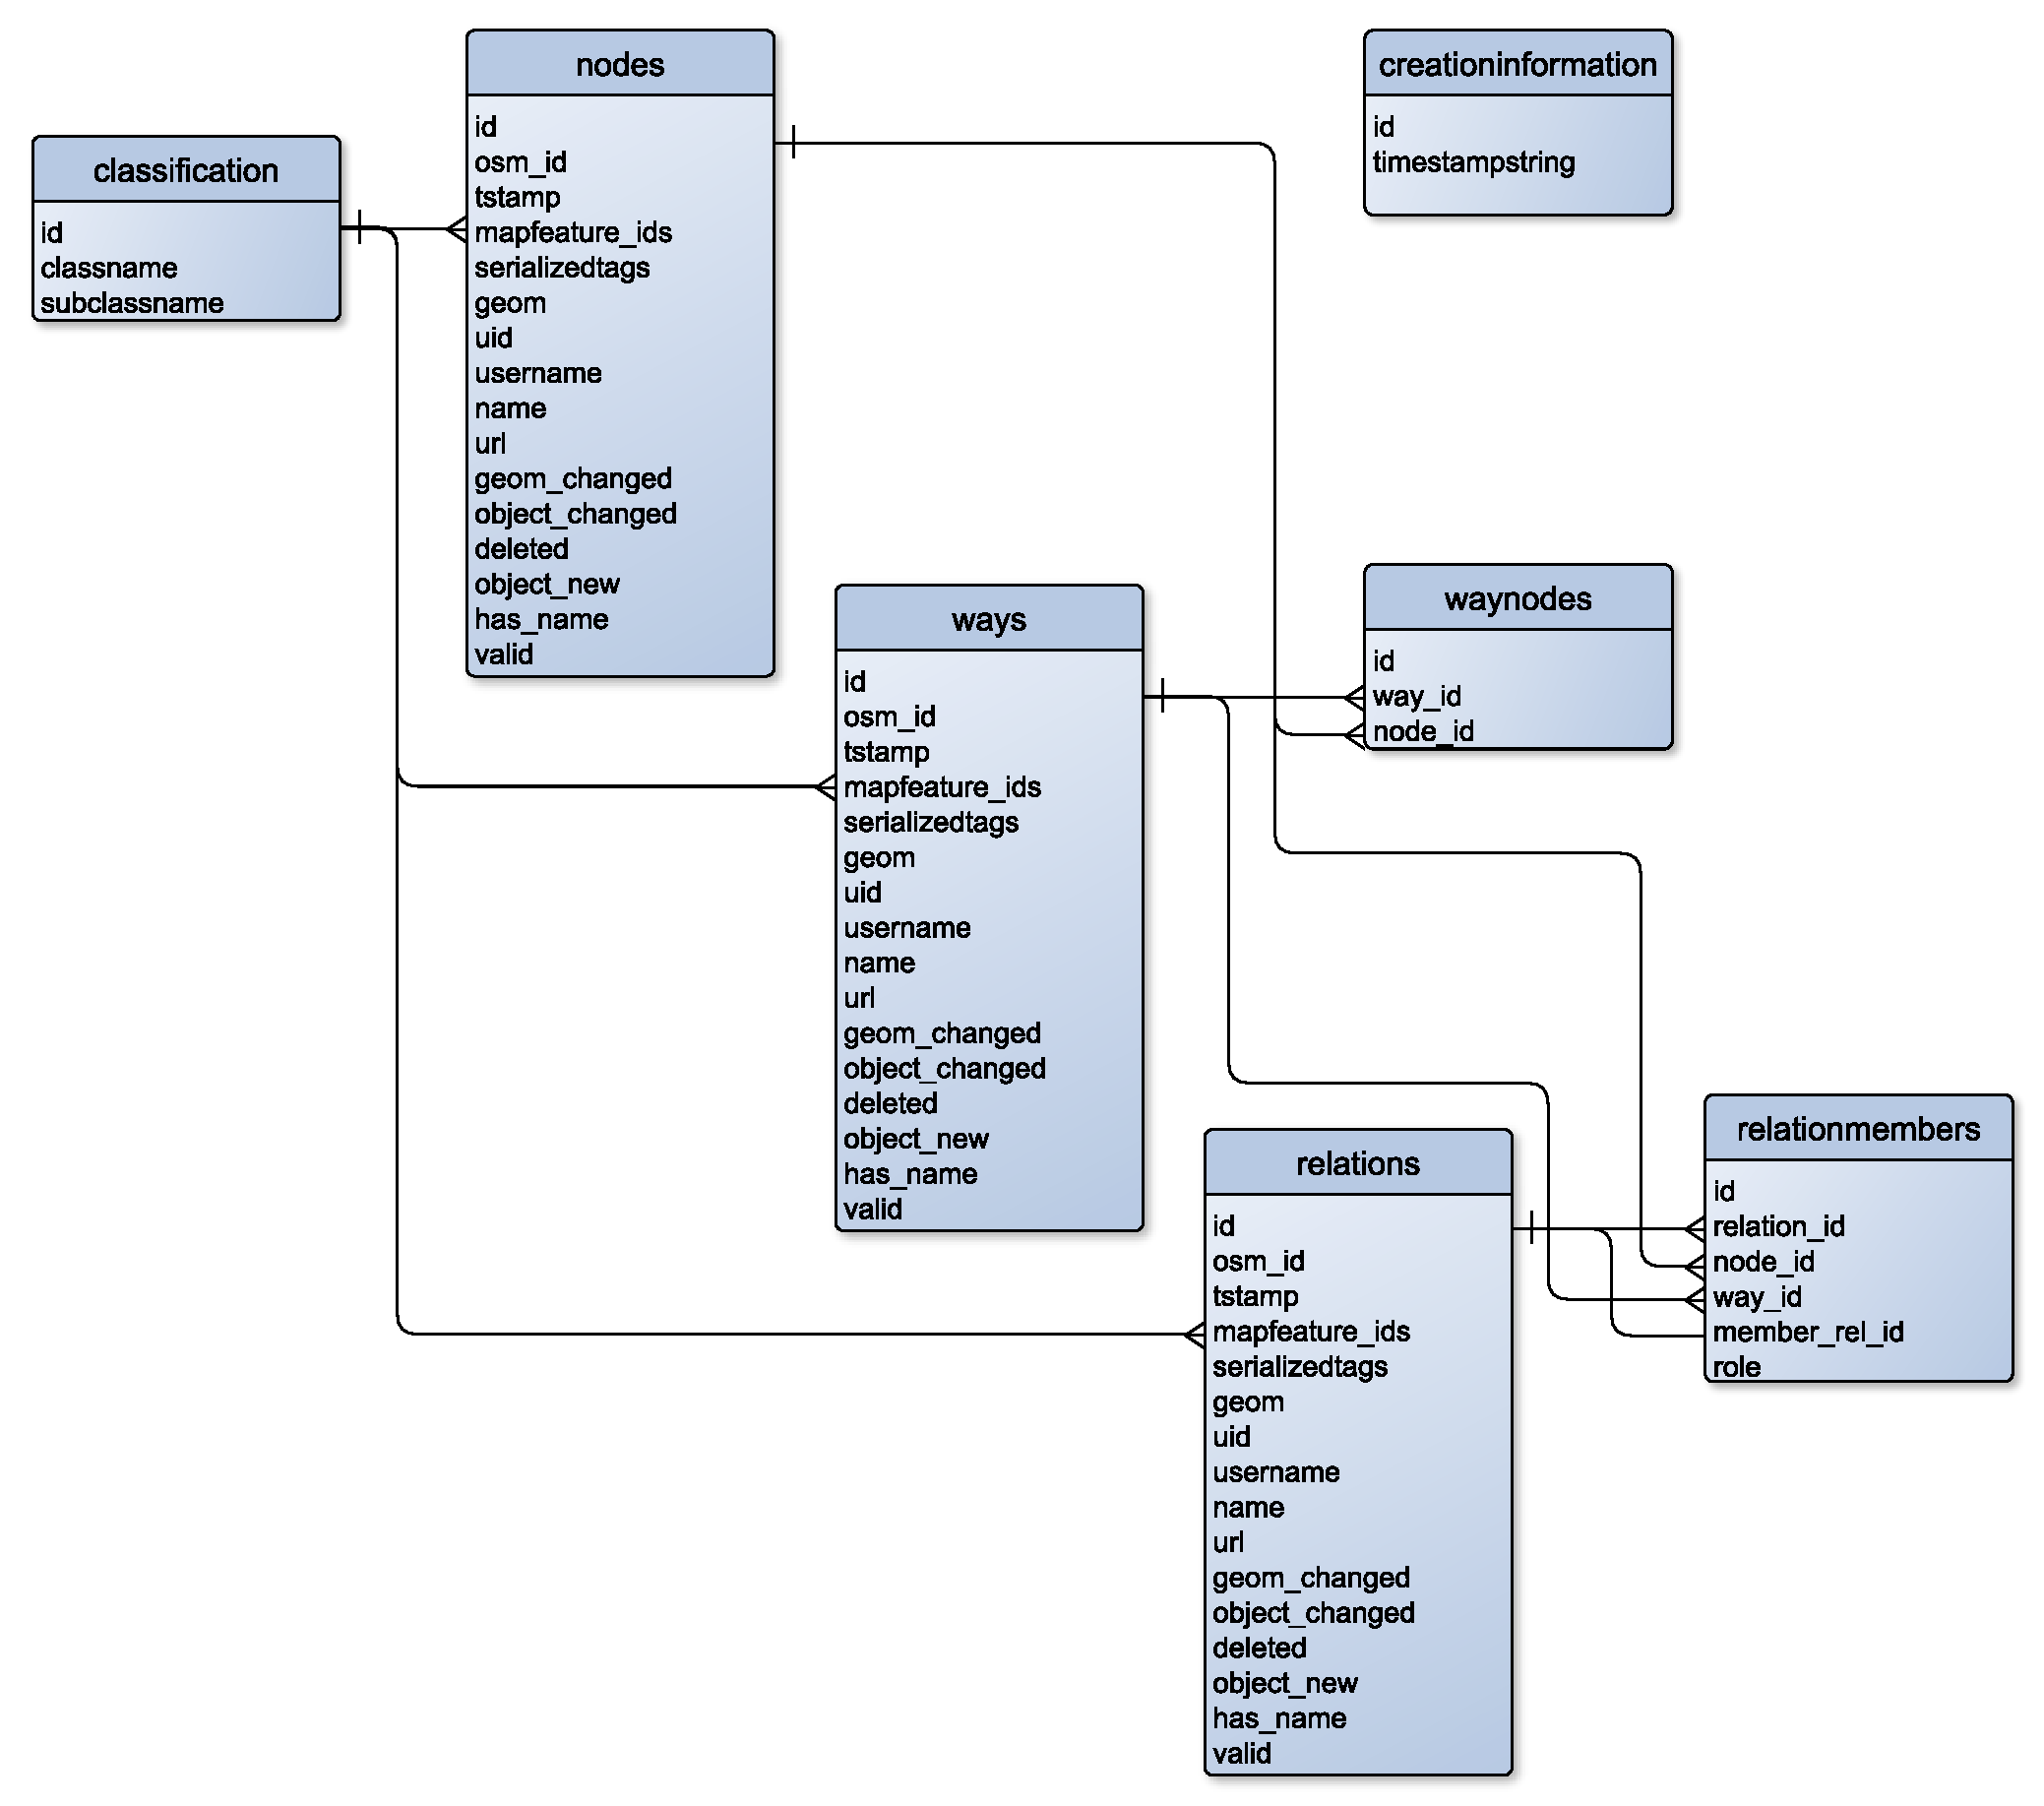
\includegraphics[width=\linewidth]{img/intermediate-db-erd.pdf}
\end{figure}

\newpage
\section{inter2ohdm}
Die Konvertierung der \gls{inter} Datenbank soll mithilfe von SQL Scripts realisiert werden. Hierbei soll, wenn möglich das Tool \gequote{\gls{psql}}\cite{postgres-psql} eingesetzt werden.

\begin{figure}[h]
	\caption{Entity Realtionship Diagramm der \gls{ohdm} Datenbank}
	\label{fig:erd-ohdm}
	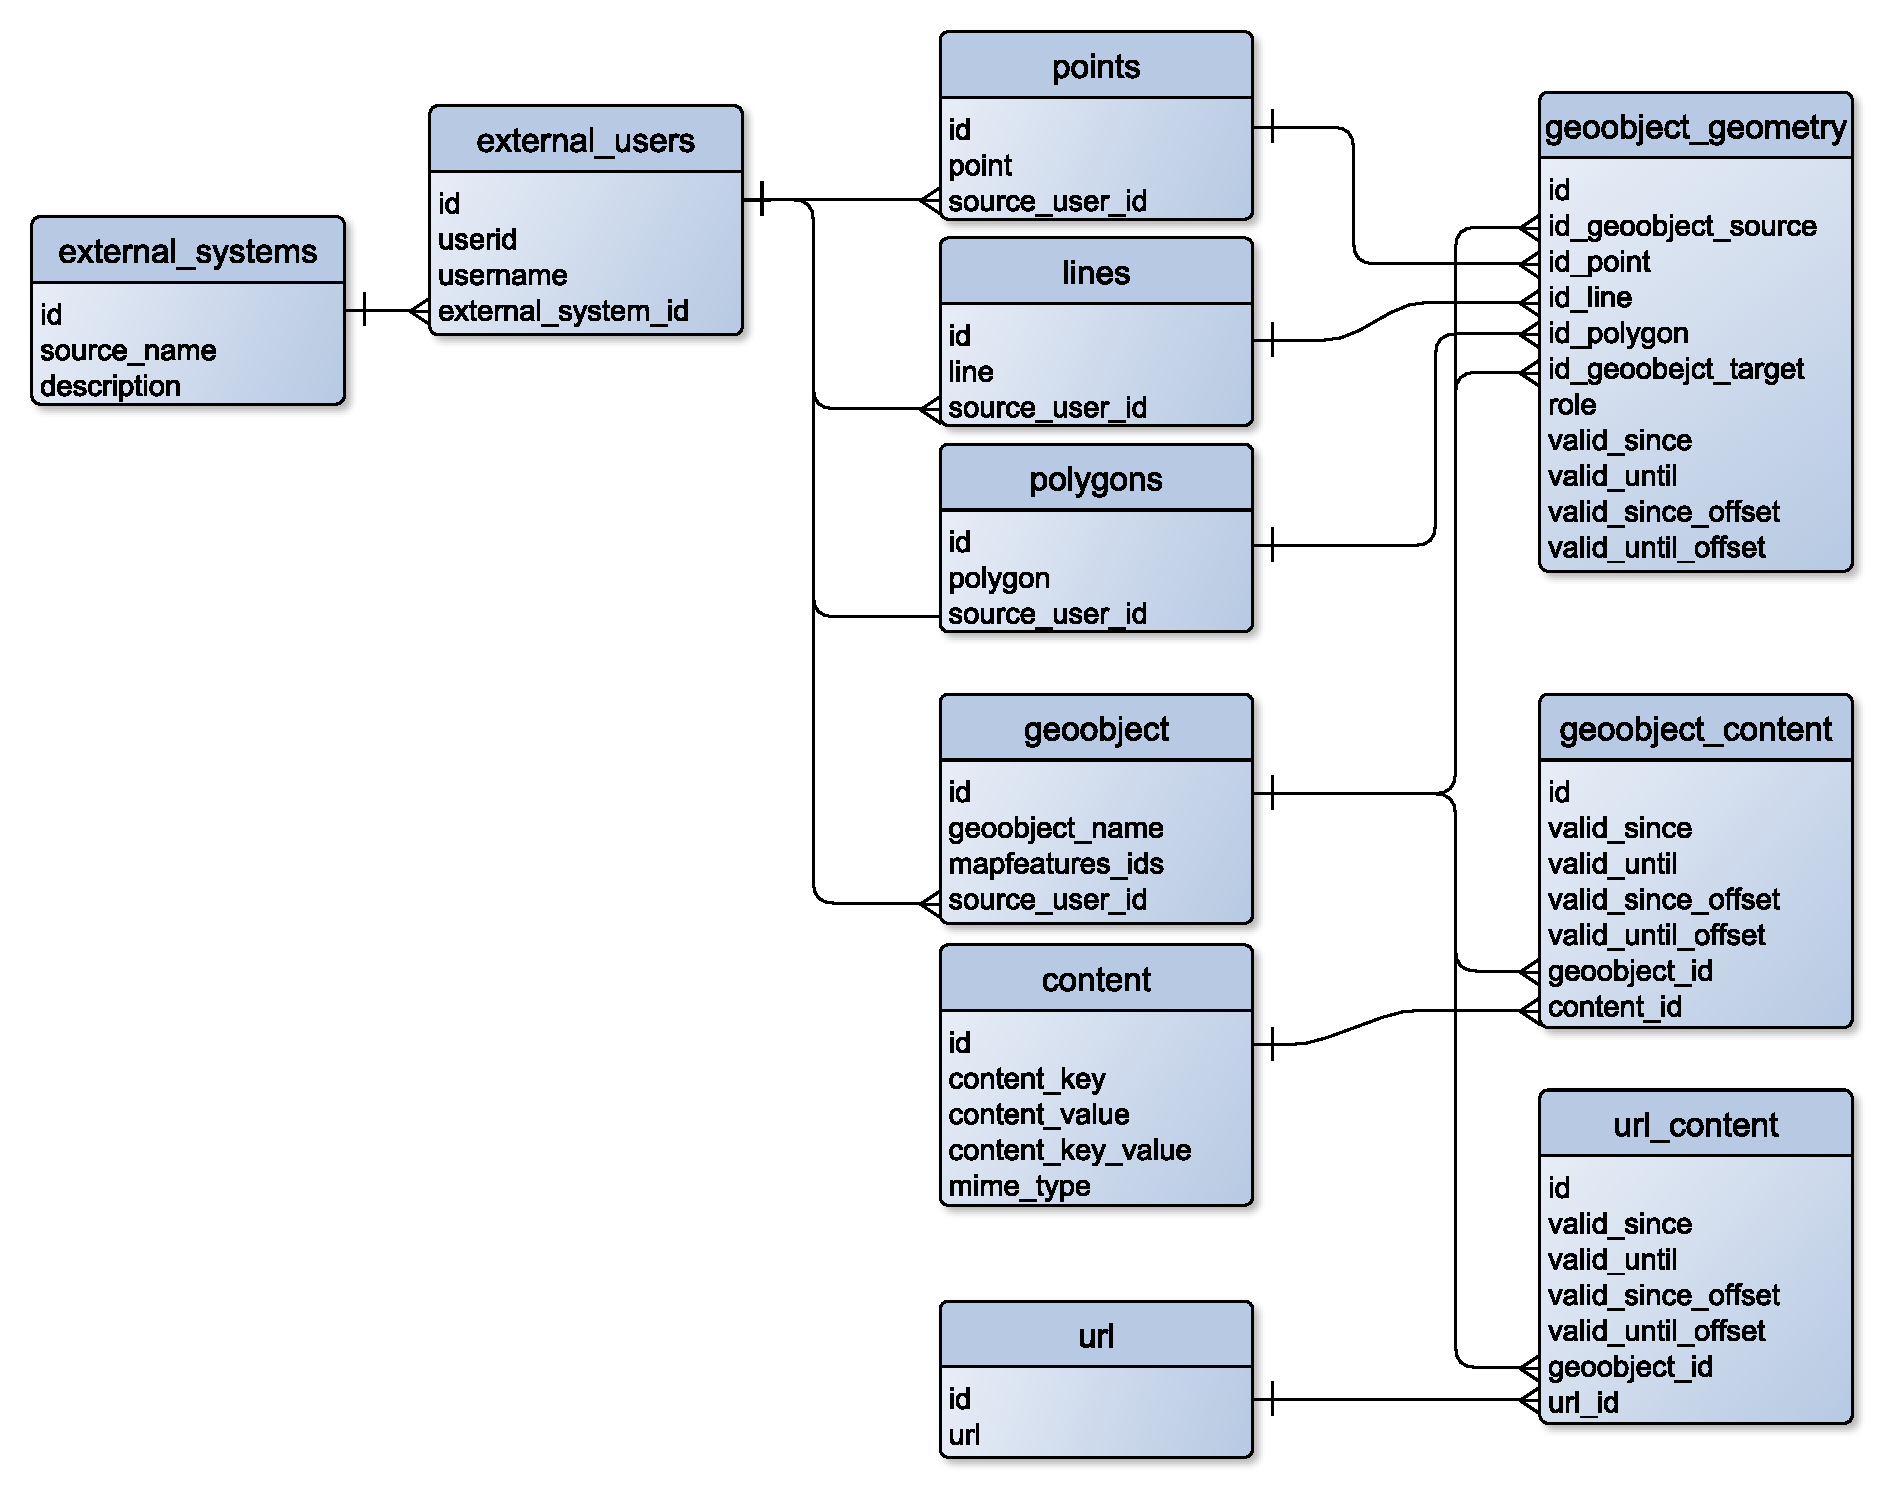
\includegraphics[width=\linewidth]{img/ohdm-db-erd.pdf}
\end{figure}

\section{Zusammenfassung}
Die beiden Datenbankschemata \gls{inter} (vgl. \autoref{fig:erd-inter}) und \gls{ohdm} (vgl. \autoref{fig:erd-ohdm}) sollen beibehalten werden. Allerdings soll jetzt mehr mit den Bordmittel von \gls{osm} und PostgreSQL gearbeitet werden.\\

Die neue Projektidee musste mit bestehenden Datenstrukturen arbeiten, da sonst auch alle anderen Teilprojekte einer Anpassung bedurften.

\chapter{osm2pgsql}
\section{Intro}
Als Importkomponente kann osm2pgsql\cite{osm2pgsql-manual} sehr vielseitig eingesetzt werden. Innerhalb des Projektes löst osm2pgsql den \gls{ohdmconverter} zum importieren von \gls{osm} in die \gls{inter} Datenbank ab. Zusätzlich lassen sich mit dem osm2pgsql nicht nur XML basierte \gls{osm} Dateien importieren sondern auch PBF und BZ2 Container. Allgemein sind \gls{pbf} Datei zu bevorzugen, da sie nur ungefähr halb so groß, wie die XML basierenden \gls{osm} Dateien sind.\cite{osm:pbf}\\

Den größten Vorteil von osm2pgsql bietet die Benutzung des \gequote{\gls{flexoutput}}. Hierbei wird die Konvertierung mit einem Lua Script angepasst.\\

Die Installation kann auf dem GitHub Repository über die \href{https://github.com/OpenHistoricalDataMap/OHDMConverter/tree/SteSad#readme}{Readme.md} eingesehen werden.

\section{osm2pgsql Flags}
Für den fehlerfreien Import sind mehrere Flags notwendig. In der nachfolgenden \autoref{tb:osm2pgsql-flags} sind diese einzeln aufgelistet mit einer entsprechenden Erklärung.
\begin{table}[h]
	\caption{Flags}
	\label{tb:osm2pgsql-flags}
	\renewcommand{\arraystretch}{1.2}
	\begin{tabularx}{\linewidth}{|l|X|}\hline
		\textbf{Flag} & \textbf{Beschreibung}\\\hline
		-H, \texttt{-{}-}host=HOST & Hostname des Datenbankservers oder Standort des Unix-Domänen-Sockets\\\hline
		-P, \texttt{-{}-}port=PORT & Port des Datenbank-Servers\\\hline
		-U, \texttt{-{}-}user=USERNAME & Datenbank-Benutzer\\\hline
		-W, \texttt{-{}-}password & Passwortabfrage erzwingen\\\hline
		-d, \texttt{-{}-}database=DB & Datenbankname oder PostgreSQL Konnektivitätsstring\\\hline
		\texttt{-{}-}log-level=LEVEL & Einstellen der Protokollstufe (debug, info (default), warn, or error)\\\hline
		-x, \texttt{-{}-}extra-attributes & Attribute (Benutzername, Benutzerkennung, Änderungssatzkennung, Zeitstempel und Version) einschließen\\\hline
		-O, \texttt{-{}-}output=OUTPUT & Spezifiziert den Output z.B.: flex, pgsql (Standard), gazetteer und null\\\hline
		-S, \texttt{-{}-}style=STYLE &  Dies gibt an, wie die Daten in die Datenbank importiert werden, ihr Format hängt von der Ausgabe ab.\newline In diesem Flag muss das Lua Script angegeben werden\\\hline		
		-c, \texttt{-{}-}create & Spezifiziert die osm Datei\\\hline
	\end{tabularx}\vspace{0.5cm}
\end{table}

\newpage
\section{Lua Script}
Für den Import in das bestehende \gls{inter} Schema wird ein Lua Script benötigt, welches den Import von \gls{osm} Daten in die \gls{inter} Datenbank spezifiziert.\\
Für eine bessere Erklärung wird das Lua Script in drei Abschnitte unterteilen:
\begin{enumerate}
	\item Tabelleninitialisierung
	\item Hilfsfunktionen und Variablen
	\item Prozessfunktionen
\end{enumerate}
Diese Beschreibung ist projektspezifisch, weitere Informationen zur Verwendung des Lua Script können unter folgendem Link eingesehen werden: \\
\url{https://osm2pgsql.org/doc/manual.html#the-flex-output}
\subsection{Tabelleninitialisierung}\label{subsec:table-init}
Im Lua Script werden erforderliche Tabellen wie in \autoref{lst:table-init-nodes} angelegt. Dies wird benötigt um die Tabelle zu spezifizieren.
\begin{lstlisting}[language={[5.0]Lua}, caption={Initialisierung eine Tabelle für alle nodes},label={lst:table-init-nodes}]
	tables.nodes = osm2pgsql.define_table({
		name = 'nodes',						
		ids = { type = 'node', id_column = 'osm_id' },
		columns = {
			{ column = 'id', sql_type = 'bigserial', create_only = true },
			{ column = 'tstamp', sql_type = 'timestamp' },
			{ column = 'mapfeature_ids', type = 'text' },
			{ column = 'serializedtags', type = 'hstore' },
			{ column = 'geom', type = 'point', projection = 4326 },
			{ column = 'uid', type = 'text' },
			{ column = 'username', type = 'text' },
			{ column = 'name', type = 'text' },
			{ column = 'url', type = 'text' },
			{ column = 'geom_changed', type = 'bool' },
			{ column = 'object_changed', type = 'bool' },
			{ column = 'deleted', type = 'bool' },
			{ column = 'object_new', type = 'bool' },
			{ column = 'has_name', type = 'bool' },
			{ column = 'valid', type = 'bool' }
		},
		schema = SCHEMA_NAME
	})
\end{lstlisting}
\autoref{lst:table-init-nodes} Zeile 4 spezifiziert den osm Typ für den die Tabelle angelegt werden soll (in dem Fall, für alle nodes) und die ID der node wird in die Spalte \gequote{osm\_id} eingetragen.\\
Zeile 6 erzeugt eine Spalte mit einem eindeutigem Integer Wert, welcher mit einem weiteren SQL Script in einen \gequote{Primary Key} verändert werden kann.\\
Die Einträge Zeile 7 - 20 definieren die weiteren Spalten der Tabelle \gequote{nodes}, welche mit einer Prozess Funktion beschrieben werden.\\
Des Weiteren kann wie in Zeile 22 ein Schema definiert werden, in die diese Tabelle geschrieben wird.

\subsection{Hilfsfunktionen und Variablen}
\subsubsection{Map Features}
\begin{lstlisting}[language={[5.0]Lua}, caption={Deklaration einer Lua Tabelle für die mapfeatures},label={lst:table-mapfeatures}]
	local map_features = {
		'admin_level', 'aerialway', 'aeroway', 'amenity', 'barrier', 'boundary',
		'building', 'craft', 'emergency', 'geological', 'healthcare', 'highway',
		'historic', 'landuse', 'leisure', 'man_made', 'military', 'natural',
		'office', 'place', 'power', 'public_transport', 'railway', 'route',
		'shop', 'sport', 'telecom', 'tourism', 'water', 'waterway'
	}
\end{lstlisting}
In \autoref{lst:table-mapfeatures} werden die sogenannten \gequote{\gls{mapfeatures}}\cite{osm-mapfeatures} definiert. \\
OpenStreetMap stellt physische Merkmale am Boden (z. B. Straßen oder Gebäude) mithilfe von Tags dar, die an seine grundlegenden Datenstrukturen (nodes, ways und relations) angehängt sind. Jedes Tag beschreibt ein geografisches Attribut des Features, das von diesem bestimmten nodes, ways oder dieser relations angezeigt wird.\\

Der aktuelle Stand beschriebt zusätzlich im Lua Script eine CSV importiert Tabelle der händisch inserierten Map Features. \\(mehr Ideen: \autoref{ap:ch:curl-mapfeatures})


\subsubsection{Hilfsfunktion für name, mapfeatures, serializedtags und url}\label{subsubsec:get.quadruple}
Die Hilfsfunktion in \autoref{lst:get-quadruple} (nächste Seite) analysiert das übergebene Objekt und gibt vier Werte zurück.
\begin{description}
	\item[name] Der primäre Name: im allgemeinen der prominenteste ausgeschilderte Name oder der gebräuchlichste Name in der/den Landessprache(n). 
	\item[mapfeatures] Eine Lua Tabelle, welche ein key-value Paar enthält. Diese Tabelle enthält alle tags welche eine Übereinstimmung mit der \lstinline|map_features| Lua Tabelle (siehe \autoref{lst:table-mapfeatures}) haben. Der Rückgabetyp ist ein String, der alle IDs der classification Tabelle, Semikolon separiert, enthält.
	\item[serializedtags] Eine Lua Tabelle mit alle object.tags, welche nicht direkt für die weitere Konvertierung benötigt werden.
	\item[url] Bei der Analyse der osm Dateien wurde festgestellt, dass eine url beziehungsweise Websitenreferenz auf verschiedene Arten eingetragen werden kann. Dieses Problem wurde ebenfalls mit der Hilfsfunktion \lstinline| get_tag_quadruple()| realisiert.
\end{description}
Der \textit{goto} Befehl entspricht in diesem Beispiel dem \textit{continue} in Java.\\
Zusätzlich dienen die Zeilen 23 - 42 der Vereinfachung der Tabelleneinträge. Alle Variablen die \lstinline|nil| sind werden in PostgreSQL mit \lstinline|NULL| eingetragen, somit entfällt eine String Vergleich um leere Einträge zu finden. Es kann direkt nach \lstinline|ISNULL| oder \lstinline|NOTNULL| im SQL Statement gefragt werden.

\newpage\begin{lstlisting}[language={[5.0]Lua}, caption={Hilfsfunktion zur osm object.tag Verarbeitung},label={lst:get-quadruple}]
	local function get_tag_quadruple(object)
	-- table with classcodes from the mapfeatures
	local features = {}
	-- declation with one entry '-1' when the osm object has not a mapfeature
	table.insert(features, '-1')
	local ser = {}
	local url = nil
	local name = object:grab_tag('name')
	-- Iterate over each tag from the osm object
	for key, value in pairs(object.tags) do
		-- find url or website entry
		if key == 'url' then
			url = object:grab_tag(key)
			goto continue
		elseif key == 'website' then
			url = object:grab_tag(key)
			goto continue
		elseif osm2pgsql.has_suffix(key, ':url') then
			url = object:grab_tag(key)
			goto continue
		elseif osm2pgsql.has_suffix(key, ':website') then
			url = object:grab_tag(key)
			goto continue
		end
	
		if list_contains(map_features, key) then
			-- osm object.tag is definied as a mapfeature
			features = get_classcode(key, value, features)
			goto continue
		else
			-- osm object.tag is not very relevant,
			-- therefore it is stored in serializedtags table
			ser[key] = value
			goto continue
		end
		:: continue ::
		end
		-- If the table is empty, an empty table should not be saved.
		-- Instead, the value is set to nil (PostgreSQL NULL)
		if next(ser) == nil then
			ser = nil
		end
	-- to save the Lua table as text in PostgreSQL Database,
	-- the table entries concat with ';' as delimiter
	return name, table.concat(features, ';'), url, ser
end
\end{lstlisting}

\newpage
\subsection{Prozessfunktionen}
Damit die nodes, ways, relations spezifisch in die gewünschten Tabellen eingetragen werden, müssen die Lua Funktionen \lstinline|osm2pgsql.process_node| \lstinline|osm2pgsql.process_way| \lstinline|osm2pgsql.process_relation| entsprechend aufgerufen werden. \\
Beispielhaft wurde die definierte Funktion \lstinline|osm2pgsql.process_relation| siehe nächste Seite in \autoref{lst:process-relation} aufgeführt.
Diese enthält:
\begin{table}[h]
	\caption{Kurze Zeilen Beschreibung von \autoref{lst:process-relation}}
	\renewcommand{\arraystretch}{1.2}
	\begin{tabularx}{\linewidth}{|l|l|X|}\hline
		Name & \multirow{2}{*}{\parbox{1.6cm}{Zeilen-\\ nummern}} & Beschreibung\\
		&& \\\hline
		\lstinline|get_tag_quadruple()| & 2 & Erstellung von vier Variablen mit einer Hilfsfunktion (siehe \autoref{subsubsec:get.quadruple})\\\hline
		\lstinline|tables.relations:add_row()| & 3-18 & Fügt ein osm Objekt entsprechend der Tabelleninitialisierung (beispielhaft \autoref{subsec:table-init}) in eine Tabelle ein. \newline Hierbei wird die id automatisch vergeben und eine Geometrie anhand der Bestehenden Daten erzeugt.\\\hline
		Schleife über alle relationmembers & 19-49 & Alle nodes, ways, relations, die im tag \textit{members} vermerkt sind werden in eine seperate Tabelle \textit{relationmembers} eingetragen. Für die Eindeutigkeit wird der Typ des \textit{members} abgefragt. \\\hline
	\end{tabularx}
\end{table}

Die Prozessfunktionen für nodes und ways sieht ähnliches aus, mit dem Unterschied, dass die \lstinline|osm2pgsql.process_node| Funktion keine zusätzlichen \textit{members} besitzt und in \lstinline|osm2pgsql.process_way| die Einträge der ways nur aus nodes bestehen.

\newpage\begin{lstlisting}[language={[5.0]Lua}, caption={Hilfsfunktion zur osm object.tag Verarbeitung},label={lst:process-relation}]
	function osm2pgsql.process_relation(object)
	local object_name, object_features, object_url, object_serializedtags = get_tag_quadruple(object)
	
	tables.relations:add_row({
		name = object_name,
		url = object_url,
		tstamp = reformat_date(object.timestamp),
		mapfeatures = object_features,
		serializedtags = object_serializedtags,
		geom = { create = 'area' },
		uid = object.uid,
		username = object.user,
		geom_changed = false,
		object_changed = false,
		deleted = false,
		object_new = false,
		has_name = false,
		valid = false
	})
	for _, member in ipairs(object.members) do
		-- if type is a node
		if member.type == "n" then
			tables.relationmembers:add_row({
				relation_id = object.id,
				node_id = member.ref,
				way_id = nil,
				member_rel_id = nil,
				role = member.role
			})
		end
		-- if type is a way
		if member.type == "w" then
			tables.relationmembers:add_row({
				relation_id = object.id,
				node_id = nil,
				way_id = member.ref,
				member_rel_id = nil,
				role = member.role
			})
		end
		-- if type is a relation
		if member.type == "r" then
			tables.relationmembers:add_row({
				relation_id = object.id,
				node_id = nil,
				way_id = nil,
				member_rel_id = member.ref,
				role = member.role
			})
		end
	end
end
\end{lstlisting}


\newpage
\section{Ausführung}
Alle vorherigen Sektionen beschreiben die wichtigen Teile des Befehls zum Import von \gls{osm} Daten in die \gls{inter} Datenbank. Der Prozess des Importes kann nun wie folgt ausgeführt werden.
\begin{lstlisting}[language={},basicstyle=\ttfamily,caption={Beispiel eines \gequote{osm2pgsql} Befehls mit dem osm2inter.lua Skript und dem Minimalbeispieldaten littlemap.osm}]
	osm2pgsql \
	--host=localhost \
	--port=5432 \
	--user=postgres \
	--password \
	--database=ohdm \
	--log-level=info \
	--extra-attributes \
	--output=flex \
	--style=/osm2inter/osm2inter.lua \
	--create /osm2inter/littlemap.osm
\end{lstlisting}
\textbf{Hinweis:} Die Dateien müssen mit absoluten Pfaden angegeben werden, oder im Verzeichnis des Datenbanknutzers gespeichert werden.\\

\chapter{psql}
psql ist ein terminalbasiertes Frontend für PostgreSQL. Es ermöglicht Ihnen, Abfragen interaktiv einzugeben, sie an PostgreSQL auszugeben und die Abfrageergebnisse anzuzeigen. Alternativ kann die Eingabe aus einer Datei erfolgen. Darüber hinaus bietet es eine Reihe von Meta-Befehlen und verschiedene shell-ähnliche Funktionen, um das Schreiben von Skripten und die Automatisierung einer Vielzahl von Aufgaben zu erleichtern.\cite{postgres-psql}

Für die Ausführung von psql werden in diesem Beispiel Flags benötigt die in \autoref{tb:psql-flags} aufgeführt sind.
\begin{table}[h]
	\caption{flags}
	\label{tb:psql-flags}
	\renewcommand{\arraystretch}{1.5}
	\begin{tabularx}{\linewidth}{|l|X|}\hline
		\textbf{Flag} & \textbf{Beschreibung}\\\hline
		-H, \texttt{-{}-}host=HOST & Hostname des Datenbankservers oder Standort des Unix-Domänen-Sockets\\\hline
		-P, \texttt{-{}-}port=PORT & Port des Datenbank-Servers\\\hline
		-U, \texttt{-{}-}user=USERNAME & Datenbank-Benutzer\\\hline
		-W, \texttt{-{}-}password & Passwortabfrage erzwingen\\\hline
		-d, \texttt{-{}-}dbname=DB & Datenbankname oder PostgreSQL Konnektivitätsstring\\\hline
		
		-c , \texttt{-{}-}command=command & Spezifiziert den ausführbaren Kommandostring\\\hline
		-f, \texttt{-{}-}file=filename & Ermöglich die Verwendung von Dateien als Quelle für Befehle.\\\hline
	\end{tabularx}\vspace{0.5cm}
\end{table}
\begin{lstlisting}[language={},basicstyle=\ttfamily,caption={Beispiel eines \gequote{psql} Befehls mit dem postprocess.sql Skript}]
	psql \
	--host=localhost \
	--port=5432 \
	--username=postgres \
	--password \
	--dbname=ohdm \
	--file=/osm2inter/osm2inter_postprocess.sql
\end{lstlisting}
\textbf{Hinweis:} Die Dateien müssen mit absoluten Pfaden angegeben werden, oder im Verzeichnis des Datenbanknutzers gespeichert werden.\\

\chapter{OHDM}
Die Konvertierung wird ausschließlich mit einem PostgreSQL Scripts realisiert\footnote{Link zum PostgreSQL Script im OHDMConverter Reporitory\\ \url{https://github.com/OpenHistoricalDataMap/OHDMConverter/blob/SteSad/inter2ohdm/inter2ohdm.sql}}, das mit psql\cite{postgres-psql} gelesen wird. Nachfolgend wird diese Script in drei Teile gesplittet.

\section{Tabellen}
\begin{figure}[h]
	\caption{OHDM Entity Relationship Modell}
	\label{fig:ohdm-erd}
	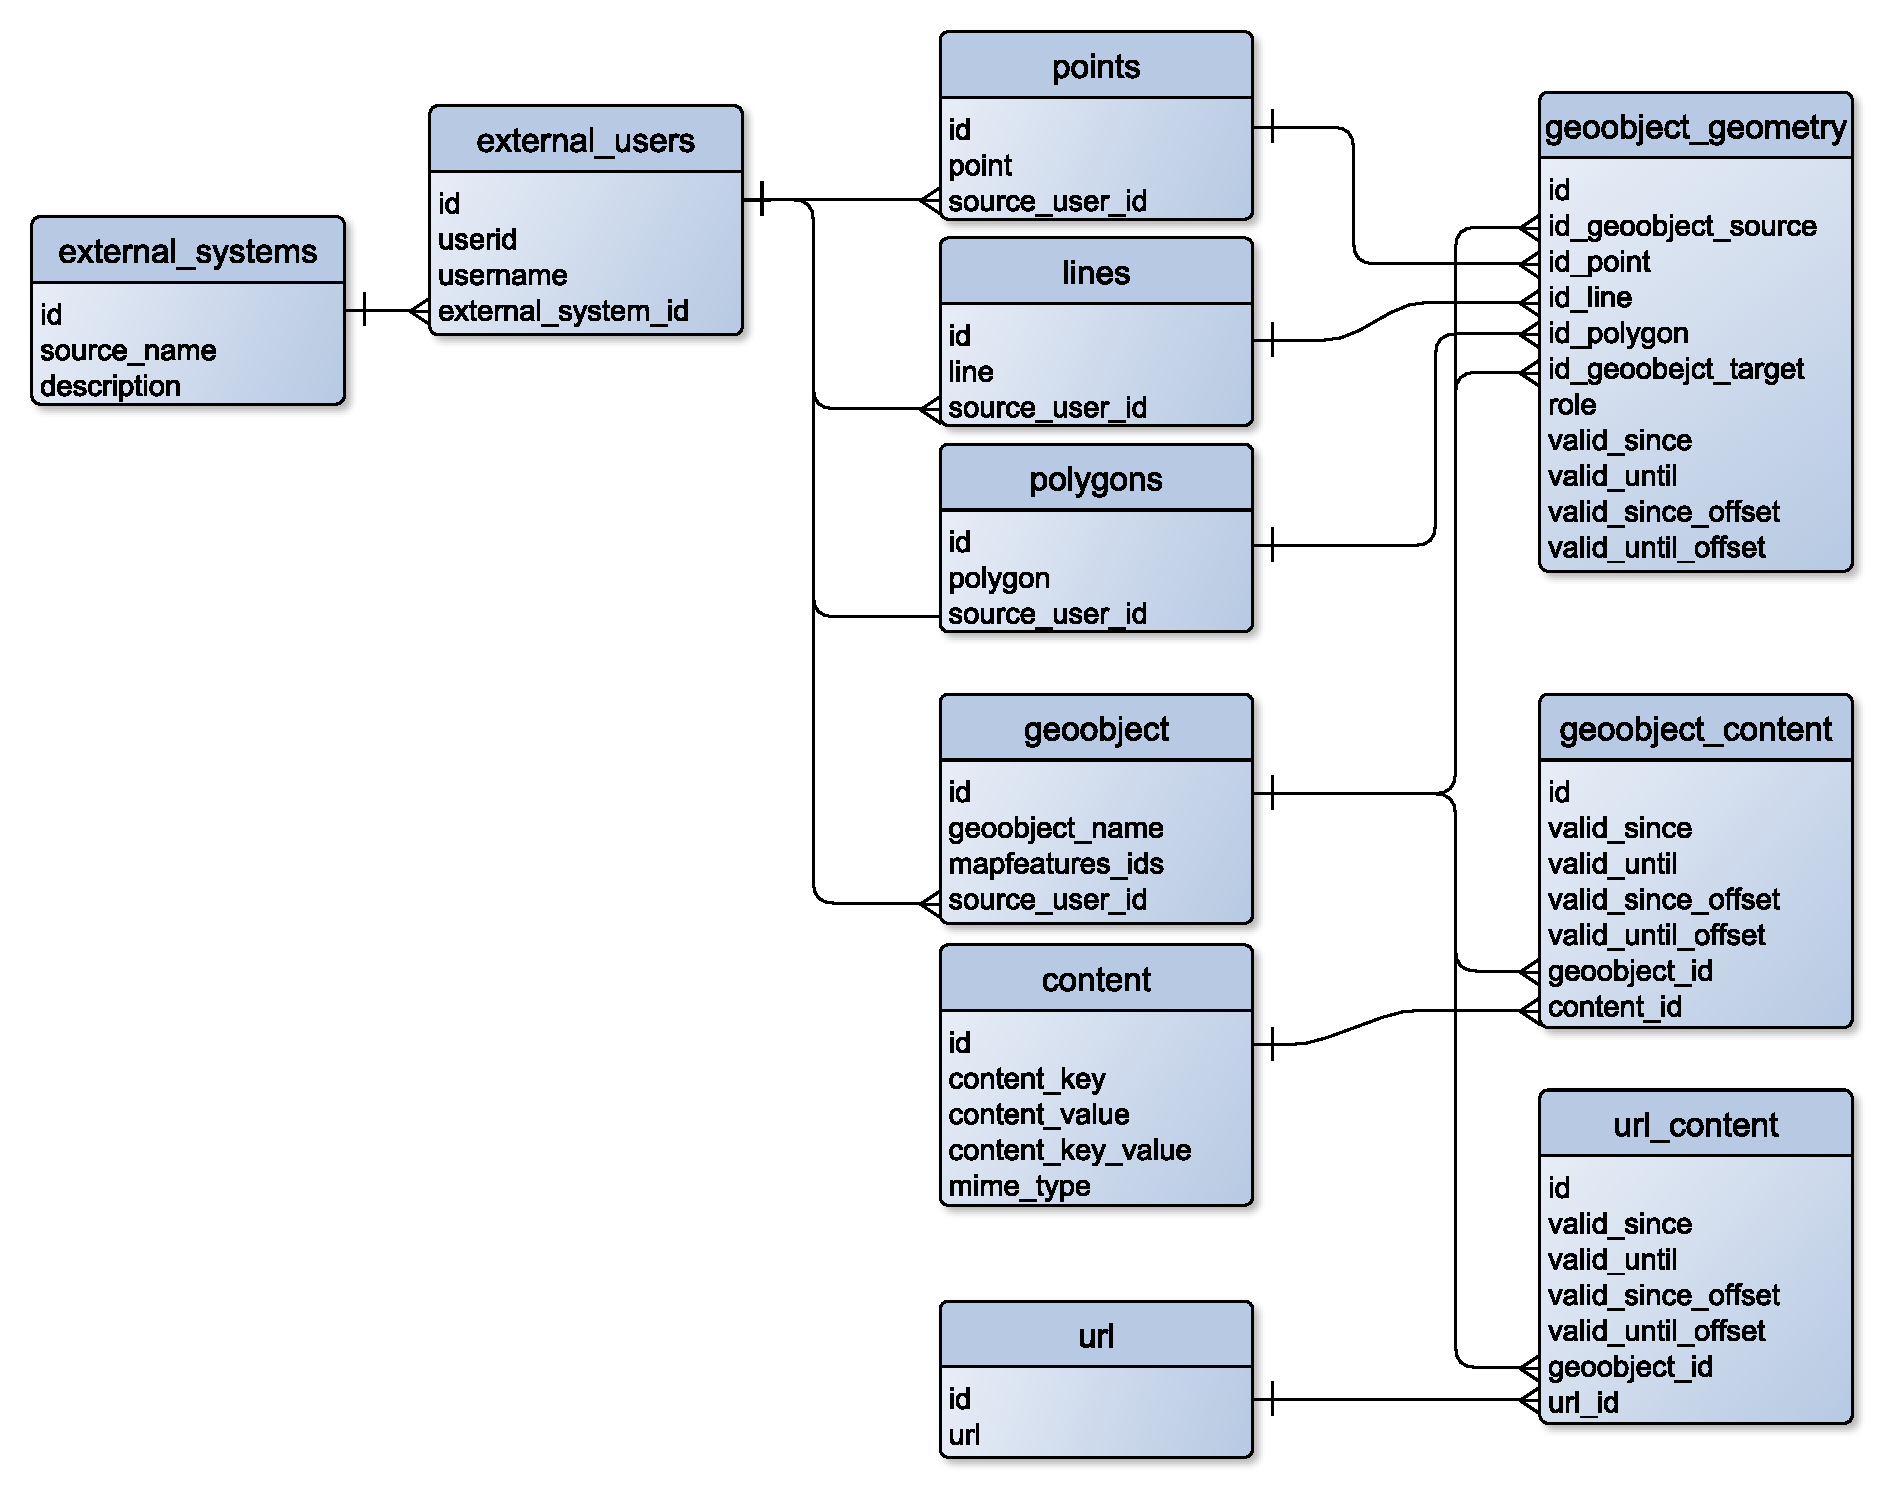
\includegraphics[width=\linewidth]{img/ohdm-db-erd.pdf}
	\caption*{gleich der \autoref{fig:erd-ohdm}}
\end{figure}

Im ersten Teil des PostgreSQL Scriptes werden alle Tabellen (siehe \autoref{fig:ohdm-erd}) erzeugt, die Spaltennamen gesetzt mit deren Datenbankvariablentypen und die Primärschlüssel Eigenschaften eingetragen. Beispielhaft für diesen Vorgang ist in \autoref{lst:sql-create-geoobject-geometry} zu sehen, wie die Tabelle \gequote{geoobject\_geometry} initialisiert wird.\newpage

\begin{lstlisting}[language=SQL,caption={Erzeugung der \gequote{geoobject\_geometry} Tabelle},label={lst:sql-create-geoobject-geometry}]
	CREATE TABLE IF NOT EXISTS ohdm.geoobject_geometry
	(
		id                  BIGSERIAL NOT NULL,
		id_geoobject_source BIGINT,
		id_point            BIGINT,
		id_line             BIGINT,
		id_polygon          BIGINT,
		id_geoobject_target BIGINT,
		role                VARCHAR,
		valid_since         DATE,
		valid_until         DATE,
		valid_since_offset  BIGINT,
		valid_until_offset  BIGINT,
		CONSTRAINT geoobject_geometry_pkey PRIMARY KEY (id)
	);
\end{lstlisting}


\section{Einfacher Insert}
Mehrere Tabellen werden mit simplen SQL Queries initialisiert. Im Beipsiel der Tabelle \gequote{external\_users} werden lediglich die Tabelleneinträge von allen \textit{nodes}, \textit{ways} und \textit{relations} vereinigt. Diese Vereinigungsmenge enthält alle Einträge, die zur Initialisierung der \gequote{external\_users} Tabelle benötigt werden. (vgl. \autoref{lst:insert-users})

\begin{lstlisting}[language=SQL,caption={Insert Statement für die \gequote{external\_users} Tabelle},label={lst:insert-users}]
	INSERT INTO ohdm.external_users(userid, username) 
	(
		SELECT uid::BIGINT, username FROM inter.nodes
		UNION
		SELECT uid::BIGINT, username FROM inter.ways
		UNION
		SELECT uid::BIGINT, username FROM inter.relations
	);
\end{lstlisting}

\newpage
\section{Join Insert}
Die meisten weiteren Initialisierungen werden mithilfe eines JOIN\footnote{vgl. \url{https://www.postgresql.org/docs/current/tutorial-join.html}} Statements realisiert. Hierbei wird eine Vereinigungsmenge gebildet, die abhänig von einer Spalte der beider zu vereinenden Tabellen ist. In \autoref{lst:insert-relation-geometry} wird eine spezielle Initialsiserung aufgezeigt, welche alle Relationen der \gls{inter} Datenbank in Verbindung mit der \gequote{relationmembers} Tabelle in die \gequote{geoobject\_geometry} Tabelle der OHDM Datenbank einfügt.

\begin{lstlisting}[language=SQL,caption={Insert Statement für die \gequote{geoobject\_geometry} Tabelle} auf Basis von allen Realationen der \gls{inter} Datenbank,label={lst:insert-relation-geometry}]
	INSERT INTO ohdm.geoobject_geometry(
		id_geoobject_source, 
		id_polygon, 
		id_geoobject_target, 
		role, 
		valid_since, 
		valid_until
	)
	(
		SELECT source.id, p.id, target.id, rm.role, r.tstamp, CURRENT_TIMESTAMP
		FROM inter.relations AS r
		JOIN inter.relationmembers AS rm ON r.osm_id = rm.relation_id
		JOIN ohdm.geoobject AS source ON r.name = source.geoobject_name
		JOIN ohdm.polygons AS p ON geom = p.polygon
		JOIN inter.relations AS re ON re.osm_id = rm.way_id
		JOIN ohdm.geoobject AS target ON re.name = target.geoobject_name
	);
\end{lstlisting}